\documentclass{article} % For LaTeX2e
\usepackage{iclr2025_conference,times}
\iclrfinalcopy % final mode: print the real byline, no review ruler (set for the v0.1.1 retitle, 2026-11-23)

% Optional math commands from https://github.com/goodfeli/dlbook_notation.
\input{math_commands.tex}

\usepackage{hyperref}
\usepackage{url}
\usepackage{booktabs}
\usepackage{graphicx}

%%%%%%%%% TITLE - PLEASE UPDATE TITLE HERE
\title{Testing Input Evidence and System One Decisions in Misinformation Classification\\[2pt] \large Pre-registered Fine-Tuning of a Typed-Decision Vision-Language Model across Three Benchmarks}

\author{Ananya Saravani Ganni, Harika Etikela, Rafiul Haider, and Krishna Batula\\
Pace University\\
Analytics Capstone, Fall 2026
}

\newcommand{\fix}{\marginpar{FIX}}
\newcommand{\new}{\marginpar{NEW}}

\begin{document}

\maketitle

\begin{abstract}
%%%%%%%%% ABSTRACT %%%%%%%%%%
Multimodal misinformation is false in structurally different ways, yet benchmarking is fragmented across at least six incompatible evaluation protocols and cost disclosure is rare. This paper reports a pre-registered fine-tuning study of LAYA-Vision, a 201M-parameter typed-decision vision-language model, under a frozen protocol across MMFakeBench, NewsCLIPpings, and VERITE. On the official MMFakeBench test split, fine-tuning on 490 training examples reaches 0.6020 macro-F1, above every directly compared Protocol A fine-tuned system and below only a frontier-model agent system, with measured inference cost of about \$0.04 per 1,000 predictions. The gains are dataset-conditional: a NewsCLIPpings trained arm is null (0.5104 accuracy versus 0.5141 for the baseline), and transfer to VERITE is flat (0.3506 versus 0.3467). Methodologically, we report a metadata leakage ceiling of 0.9150 on MMFakeBench, show that a calibration temperature fitted on one distribution can severely harm held-out calibration, and provide a complete metered GPU cost ledger of approximately \$5.64 for the entire programme. All negative results are reported unsoftened.
%%%%%%%%% ABSTRACT %%%%%%%%%%
\end{abstract}

\section{Introduction}
\label{sec:intro}
%%%%%%%%% INTRODUCTION %%%%%%%%%%
Multimodal misinformation rarely lies in one modality alone. A social-media post pairs an image with a caption, and the pair can be false in structurally different ways: the text can distort facts, the image can be manipulated or miscaptioned, and two individually authentic items can be placed together out of context. A useful detector therefore needs to say not only \emph{whether} a pair is false but \emph{how} it is false. This typed-decision view connects to earlier evidence-based claim verification \citep{Thorne2018FeverLargescale, Augenstein2019MultifcRealworld, Guo2021SurveyAutomated}, to surveys that separate factuality from harm \citep{Alam2021SurveyMultimodal}, and to work on detecting and grounding manipulated media \citep{Shao2023DetectingGrounding}. Benchmarks such as MMFakeBench \citep{Liu2024MmfakebenchMixedsource}, NewsCLIPpings \citep{Luo2021NewsclippingsAutomatic}, and VERITE \citep{Papadopoulos2023VeriteRobust} operationalize this typology with different label spaces and native metrics.

This paper extends a companion study by the same team, \emph{Testing Input Evidence and System One Decisions in Misinformation Classification}, which measured how classification responds to changes in input evidence (a publisher cue removed from text, images degraded, the image modality withheld) while every model stayed frozen. That study characterised sensitivity; this one intervenes. It asks what changes when the evidence a model has internalised is itself altered, through pre-registered fine-tuning of a typed-decision vision-language model, and it reports the outcomes, positive and negative, under frozen selection rules on the same family of benchmarks. Where the companion study varied the input at evaluation time, this paper varies it at training time; the two are complementary halves of one question. Figure~\ref{fig:sard} redraws the companion study's three evidence tests together with the accuracies it reported.

\begin{figure}[t]
\centering
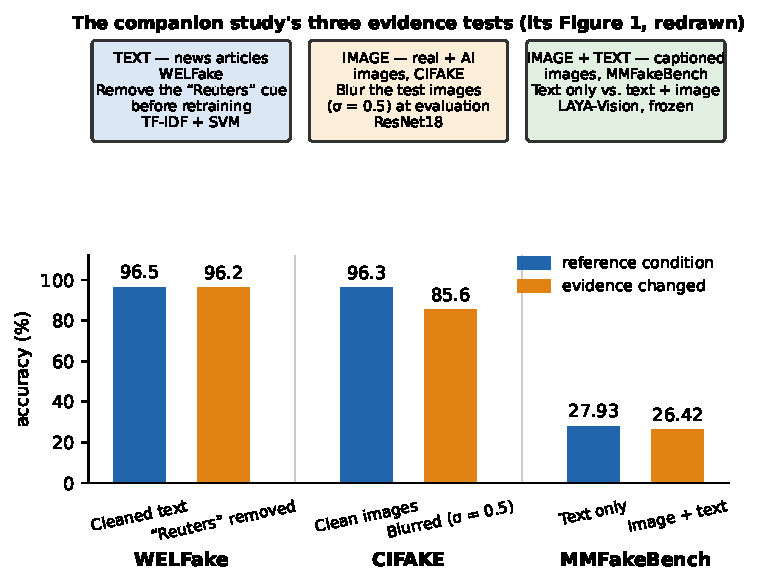
\includegraphics[width=\textwidth]{figures/fig_sard.pdf}
\caption{The companion study's three evidence tests and their accuracies. Top: the three tests as drawn in the companion study's opening figure (Seidenberg Annual Research Day (SARD), Pace University, 11 December 2026), redrawn. Bottom: accuracy in the reference condition and in the changed-evidence condition. On WELFake, a TF-IDF support vector machine scores 96.5\% on cleaned text and 96.2\% after the ``Reuters'' cue is removed; on CIFAKE, a fine-tuned ResNet18 scores 96.3\% on clean images and 85.6\% after Gaussian blur at evaluation; on MMFakeBench, frozen LAYA-Vision scores 27.93\% with text alone and 26.42\% with image and text. These are the companion study's results, measured with frozen models; this paper's own results are in Section~\ref{sec:experiments}.}
\label{fig:sard}
\end{figure}

Most current progress is dominated by large vision-language models (LVLMs) and agent frameworks. Contrastively pretrained encoders such as CLIP \citep{Radford2021LearningTransferable}, instruction-tuned assistants such as LLaVA and InstructBLIP \citep{Liu2023VisualInstruction, Dai2023InstructblipTowards}, and compact LVLMs \citep{Zhu2024LlavaphiEfficient} provide strong zero-shot image--text representations. Agent wrappers compose these models with tools and retrieval: HuggingGPT and ViperGPT turn multimodal inference into programmed tool use \citep{Shen2023HugginggptSolving, Surs2023VipergptVisual}; SNIFFER adds external evidence for explainable out-of-context detection \citep{Qi2024SnifferMultimodal}; MMD-Agent integrates reasoning and tools on MMFakeBench \citep{Liu2024MmfakebenchMixedsource}. Subsequent systems add evidence retrieval, type-aware reasoning, or test-time search; while promising, they frequently use validation, retrieval, or private re-split protocols that make their published figures difficult to compare directly. These systems often require frontier APIs, external retrieval, test-time search, or private re-splits, and operational cost is rarely disclosed.

Fine-tuned detectors offer a smaller alternative. Early multimodal fake-news systems learned shared representations or event-invariant features \citep{Khattar2019MvaeMultimodal, Wang2018EannEvent, Singhal2019SpotfakeMultimodal}; standard visual-language transformers such as LXMERT and VisualBERT remain common baselines \citep{Tan2019LxmertLearning, Li2019VisualbertSimple}. Parameter-efficient fine-tuning, especially LoRA and related low-rank recipes, makes small-data adaptation cheap \citep{Hu2021LoraLowrank, Kalajdzievski2023RankStabilization, Shuttleworth2024LoraVs}. Yet existing fine-tuned detectors often rely on larger external datasets, leave their split conventions unstated, or do not pre-register hyperparameters, which makes stability and transfer properties hard to audit.

Two further problems recur. First, evaluations leak. Dataset bias can inflate performance through annotation artifacts or metadata shortcuts \citep{Gururangan2018AnnotationArtifacts, Gebru2018DatasheetsDatasets}; leakage and reproducibility failures are widespread in machine-learning-based science \citep{Kapoor2023LeakageReproducibility, Pineau2020ImprovingReproducibility, Kapoor2024ReformsConsensusbased}. In our audit, a metadata-only rule reaches 0.9150 macro-F1 on the MMFakeBench tune split, a leakage ceiling that we report as a benchmark warning. Second, calibration is fragile: fitted temperatures are often treated as model properties even though calibration depends on the model--distribution pair \citep{Guo2017CalibrationModern, Naeini2015ObtainingWell, Ovadia2019CanYou, Minderer2021RevisitingCalibration}.

Typed-decision models are a much smaller alternative. Instead of generating free text, a typed-decision model reads a structured state plus a typed question and returns calibrated probabilities over a fixed option set in a single forward pass. LAYA-Vision, a 201M-parameter typed-decision vision-language model used in this study, follows this design. Our preceding diagnostic study found that the pretrained model does not perform multimodal misinformation detection zero-shot: it collapses onto a single class on MMFakeBench, a TF-IDF logistic baseline implemented with scikit-learn \citep{Pedregosa2011ScikitlearnMachine} roughly doubles its macro-F1, and a frozen-feature probe shows its representation carries signal that its decision head does not use.

This paper reports a pre-registered fine-tuning study of LAYA-Vision across three benchmarks whose definitions of falsity differ: MMFakeBench \citep{Liu2024MmfakebenchMixedsource}, NewsCLIPpings \citep{Luo2021NewsclippingsAutomatic}, and VERITE \citep{Papadopoulos2023VeriteRobust}. The contribution is primarily methodological: we do not introduce a new architecture or training algorithm. Instead, we show that a small typed-decision model, when embedded in a pre-registered, receipted protocol with explicit leakage and calibration checks, can yield one strong, one null, and one flat result across three benchmarks. We freeze a single protocol before evaluation: selection on tune only, the MMFakeBench test split scored exactly once, calibration fitted only on a reserved split, and all training runs receipted. The main grid compares full encoder-plus-head and LoRA arms under two objectives and three step budgets; a supplementary ablation tier runs after selection and never feeds it. Pre-registered hypotheses H1--H5 cover MMFakeBench gain, a NewsCLIPpings trained arm, VERITE transfer, per-class recall floors, and calibration.

The study yields three main results. First, on the directly comparable official MMFakeBench test protocol, a 201M model fine-tuned on 490 examples reaches 0.6020 macro-F1, with per-prediction inference cost around \$0.04 per 1,000 items and zero external dependencies. Second, the same recipe produces a null result on NewsCLIPpings (trained 0.5104 accuracy versus 0.5141 for this run's baseline) and near-flat transfer to VERITE (0.3506 versus 0.3467), showing that the gains are dataset-conditional. Third, methodological findings have independent value: a calibration temperature fitted on one distribution can harm held-out calibration, while a distribution-matched fit repairs it; a metadata leakage ceiling of 0.9150 exposes a benchmark shortcut; and the MMFakeBench literature is fragmented across at least six incompatible protocols. Throughout, we report negative results unsoftened and provide complete accounting of metered GPU cost, latency, artifact size, and deviations.

\section{Related Work}
\label{sec:related_work}
%%%%%%%%% RELATED WORK %%%%%%%%%%
We organize related work into three technical clusters: large vision-language models and agent frameworks, fine-tuned multimodal detectors and parameter-efficient fine-tuning, and calibration, dataset bias, and benchmark protocol fragmentation.

\subsection{Large Vision-Language Models and Agent Frameworks}
Large-scale contrastive pretraining, instruction tuning, and efficient multimodal assistants have reshaped image--text classification. CLIP \citep{Radford2021LearningTransferable}, LLaVA \citep{Liu2023VisualInstruction}, InstructBLIP \citep{Dai2023InstructblipTowards}, and compact LVLMs such as LLaVA-Phi \citep{Zhu2024LlavaphiEfficient} provide powerful zero-shot or instruction-following backbones. On multimodal misinformation tasks, however, the most visible recent systems wrap these models in agent loops. HuggingGPT and ViperGPT compose external tools through generated programs \citep{Shen2023HugginggptSolving, Surs2023VipergptVisual}; SNIFFER performs two-stage instruction tuning and retrieves external knowledge for out-of-context explanations \citep{Qi2024SnifferMultimodal}; MMD-Agent integrates reasoning, action, and tool use for MMFakeBench \citep{Liu2024MmfakebenchMixedsource}. Benchmarks such as MFC-Bench and LVLM studies further document sensitivity to manipulated content and evaluation design \citep{Wang2024MfcbenchBenchmarking, Tahmasebi2024MultimodalMisinformation}. These systems commonly assume frontier APIs, external retrieval, or test-time search, and their results are often reported under different split and metric regimes. Older cross-modality encoders such as LXMERT and VisualBERT remain standard comparison points on NewsCLIPpings-style data \citep{Tan2019LxmertLearning, Li2019VisualbertSimple}. Our work is not an agent system: it is a single forward-pass typed-decision classifier with zero external dependencies, and its reported costs and split labels are explicit.

\subsection{Fine-Tuned Multimodal Detectors and Parameter-Efficient Fine-Tuning}
Fine-tuned multimodal detectors predate large LVLM agents. Event-adversarial networks remove event-specific features \citep{Wang2018EannEvent}, multimodal variational autoencoders learn shared representations \citep{Khattar2019MvaeMultimodal}, and early frameworks such as SpotFake fuse BERT and VGG features without auxiliary subtasks \citep{Singhal2019SpotfakeMultimodal}. Cross-modality transformers such as LXMERT and VisualBERT provide strong baselines \citep{Tan2019LxmertLearning, Li2019VisualbertSimple}. Parameter-efficient fine-tuning (PEFT) makes adaptation cheaper. LoRA injects low-rank updates into frozen weights \citep{Hu2021LoraLowrank}; later work improves rank allocation \citep{Zhang2023AdaloraAdaptive}, analyzes learning-rate asymmetries \citep{Hayou2024LoraEfficient}, compares LoRA with full fine-tuning through spectral structure \citep{Shuttleworth2024LoraVs}, and stabilizes rank scaling \citep{Kalajdzievski2023RankStabilization}. Vector-based random-matrix adaptation further reduces parameter counts \citep{Kopiczko2023VeraVectorbased}. For vision-language models, adapter-style and training-free cache approaches improve few-shot transfer \citep{Gao2021ClipadapterBetter, Zhang2022TipadapterTrainingfree}, and unified views of visual PEFT compare these recipes \citep{Yu2022TowardsUnified}. In our study, a standard LoRA arm and a full encoder-plus-head arm are pre-registered, selected only on a tune split, and evaluated across datasets. We also report rank-stability hazards under this recipe rather than selecting the best post hoc.

\subsection{Calibration, Dataset Bias, and Benchmark Protocol Fragmentation}
Modern neural networks can be miscalibrated, and temperature scaling is a standard mitigation \citep{Guo2017CalibrationModern, Naeini2015ObtainingWell}. However, calibration is not a fixed model property: it degrades under dataset shift \citep{Ovadia2019CanYou, Minderer2021RevisitingCalibration}, which motivates distribution-aware and non-parametric calibration methods \citep{Kull2019BeyondTemperature, Kumar2019VerifiedUncertainty, Vaicenavicius2019EvaluatingModel, Gupta2020CalibrationNeural, Nixon2019MeasuringCalibration, Barber2019ConformalPrediction, Gibbs2021AdaptiveConformal}. Our experiments provide a concrete instance of this distribution dependence: a temperature fitted on one split raises held-out ECE, while a split-half fit repairs it. Dataset bias and leakage are equally important. Annotation artifacts can make label prediction possible from partial inputs \citep{Gururangan2018AnnotationArtifacts}; leakage taxonomies and reproducibility programs show how such shortcuts lead to overoptimistic conclusions \citep{Kapoor2023LeakageReproducibility, Pineau2020ImprovingReproducibility, Kapoor2024ReformsConsensusbased}. Dataset documentation standards such as datasheets support the disclosure of metadata and intended use \citep{Gebru2018DatasheetsDatasets}. In this study we report a 0.9150 metadata leakage ceiling on MMFakeBench and formally refuse to feed source metadata to the model. Finally, because benchmark scores are often averaged or transferred across tasks, we separate datasets and transfer results rather than aggregating them; this echoes the separation of average accuracy from transfer in continual-learning evaluation \citep{Lopezpaz2017GradientEpisodic}.
%%%%%%%%% RELATED WORK %%%%%%%%%%

\section{Methodology}
\label{sec:method}
%%%%%%%%% METHOD %%%%%%%%%%
\subsection{Typed-Decision Formulation and Dataset Packs}
Let an image--text pair be \(x=(t,v)\), where \(t\) is the context text and \(v\) is the image. Let \(\mathcal{Y}\) be the fixed label set of a dataset pack. A typed-decision model \(M_\theta\) maps the pair and a dataset-specific typed question \(q\) to a distribution over \(\mathcal{Y}\):
\[
p(y\mid x,q;\theta)=M_\theta(x,q),
\qquad
\hat{y}=\mathop{\mathrm{arg\,max}}_{y\in\mathcal{Y}}\,p(y\mid x,q;\theta).
\]
Every evaluation call returns two questions in one forward pass: a native choice question over the dataset's own classes, and a binary fake screen expressed as a \( \texttt{noul} \) probability question. The choice verdict is the headline; the screen is reported beside it, and disagreement between the two is labeled as uncertain.

Per-dataset packs fix the questions, label spaces, native metrics, and calibration behavior. Specifically, MMFakeBench uses four classes (original, textual veracity distortion, visual veracity distortion, mismatch) and macro-F1; NewsCLIPpings uses pristine versus falsified and accuracy; VERITE uses truthful, miscaptioned, and out-of-context and three-class accuracy. These metrics are never averaged across datasets.

Gold labels, item IDs, file paths, and source metadata are never model inputs. To measure the risk of shortcut learning, we define a metadata-only rule that reads only the two provenance fields \( \texttt{text\_source} \) and \( \texttt{image\_source} \), maps each observed source combination to the most frequent label, and predicts every item with that provenance as that label. This rule uses no image or text content. It reaches 0.9150 macro-F1 on the MMFakeBench tune split, and 0.9150 accuracy / 0.8510 macro-F1 on the official test split. We report this leakage ceiling as a benchmark warning rather than as a model result. This audit is deliberately narrow: it examines only explicit source metadata. It does not test for content-based source-identifying cues such as watermarks, text style, or image artifacts. The ceiling therefore demonstrates that a metadata-only shortcut exists; it does not quantify every possible shortcut signal in the benchmark.

\subsection{Model Architecture and Trainable Arms}
LAYA-Vision is a 201M-parameter typed-decision vision-language model with a language encoder and a two-layer decision head. The checkpoint used is \( \texttt{thaitea/laya-vision} \) at pinned revision \( \texttt{f2fe3c12cb6d04c59d8a190250bf3fb40fc828dc} \). The model does not generate free text; it returns probabilities over a fixed option set in a single forward pass. The checkpoint is used exactly as released, and fine-tuning does not modify the architecture. Figure~\ref{fig:arch} shows the computation.

\begin{figure}[t]
\centering
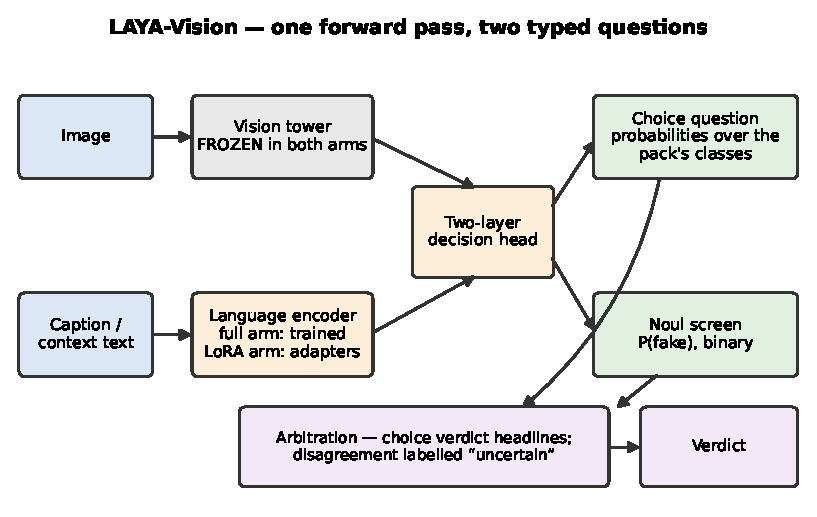
\includegraphics[width=\textwidth]{figures/fig_arch.pdf}
\caption{LAYA-Vision as used in this study. An image--text pair enters one forward pass: the vision tower is frozen in both training arms; the language encoder and the two-layer decision head are trained, directly in the full arm and through low-rank adapters in the LoRA arm; and the head answers two typed questions, a native choice question over the dataset pack's classes and a binary fake screen. The choice verdict headlines; disagreement between the two answers is labelled uncertain.}
\label{fig:arch}
\end{figure}

We compare two trainable arms. The full arm trains the language encoder and decision head, with 114,728,323 of 201,161,347 parameters trainable. The vision tower is frozen in both arms due to a library limitation; following the binding labelling rule, this arm is always described as encoder-plus-head fine-tuning, never full-model fine-tuning. The LoRA arm follows \citet{Hu2021LoraLowrank} with rank \(r=16\), scaling factor \( \alpha=32\), dropout \(0.05\), and targets the query, value, key, output, gate, up, and down projections. Its learning rate is \( \texttt{lr\_lora}=0.001\), and it is always reported as such. Rank-scaling issues are relevant because higher ranks are explored in the supplementary tier \citep{Kalajdzievski2023RankStabilization}.

\subsection{Fine-Tuning Objectives and Frozen Protocol}
The main grid uses the training library's two built-in objectives. For every dataset pack, the training library produces a fixed soft target from the pack definition. We use the pinned library implementation as the authoritative specification: we do not infer the target construction from external mathematics and do not replace it with an ad-hoc smoothing rule. Let \(p_\theta(c\mid x,q)\) be the model probability for class \(c\), and let \(\tilde{p}_{\mathrm{soft}}(c\mid x,q)\) be the library-defined soft target for the active dataset pack. The \( \texttt{soft\_ce} \) objective is
\[
\mathcal{L}_{\mathrm{soft\_ce}}(\theta)
=
-\frac{1}{n}
\sum_{i=1}^{n}
\sum_{c\in\mathcal{Y}}
\tilde{p}_{\mathrm{soft}}(c\mid x_i,q_i)
\log p_\theta(c\mid x_i,q_i),
\]
where the soft targets are fixed by the dataset pack and are not learned from any evaluation split. The \( \texttt{rlcd} \) objective is the library's built-in \( \texttt{rlcd} \) term and is likewise defined by the pinned code. Because the identity of the library's \( \texttt{rlcd} \) objective relative to published RLCD methods is unresolved, we deliberately refrain from writing an external mathematical definition for it and do not claim that it corresponds to a published RLCD loss. Every soft-ce-versus-rlcd claim is scoped as ``within this library's two objectives, under this recipe,'' never as a claim about RLCD in general.

The MMFakeBench development partition is frozen as 490 train items (980 records, with each item in both question forms), 105 tune items (210 records), and 105 calibration items (210 records). This partition is carved from the official 1,000-item MMFakeBench validation split; the official 10,000-item test split is not used for selection, calibration, or any adaptation step. Selection uses only the tune split. The MMFakeBench test split is scored exactly once, by the frozen winner, after selection. Calibration is fitted only on the reserved calibration split after selection. Gold labels, item IDs, file paths, and source metadata are never model inputs.

\subsection{Hypotheses and Evaluation Metrics}
We pre-register five binary hypotheses before evaluation.
\begin{itemize}
    \item \textbf{H1 (MMFakeBench gain):} the winning configuration improves test macro-F1 over the pretrained baseline by at least \(+0.03\), with paired-resampling 95\% CI lower bound greater than zero and no per-class recall drop larger than 5 percentage points.
    \item \textbf{H2 (NewsCLIPpings trained arm, as re-aimed by amendment (c)):} validation accuracy falls in the \(0.55\)--\(0.65\) band and improves over the October baseline \(0.5083\) by at least \(+6.24\) percentage points.
    \item \textbf{H3 (VERITE transfer):} the MMFakeBench winner, transferred without VERITE training, reaches accuracy in the \(0.38\)--\(0.48\) band.
    \item \textbf{H4 (recall floor):} the minimum per-class tune recall of the winner is at least \(0.25\).
    \item \textbf{H5 (calibration):} fitted calibration brings calibration-split expected calibration error under \(0.15\), with accuracy unchanged.
\end{itemize}

For expected calibration error, we use the standard binned estimator:
\[
\mathrm{ECE}
=
\sum_{m=1}^{M}
\frac{|B_m|}{n}
\left|
\mathrm{acc}(B_m)
-
\mathrm{conf}(B_m)
\right|,
\]
where \(B_m\) is the \(m\)-th confidence bin. Negative log-likelihood is computed as
\[
\mathrm{NLL}
=
-\frac{1}{n}
\sum_{i=1}^n
\log p(y_i\mid x_i,q;\theta).
\]
Paired resampling confidence intervals use 2,000 resamples, and differences between systems are stated in percentage points rather than as bare percent changes.

\section{Experiments}
\label{sec:experiments}
%%%%%%%%% EXPERIMENTS %%%%%%%%%%
\subsection{Experimental Setup and Cost Ledger}
Training uses seed 20261122, maximum sequence length 1024, batch size 8, and bf16 precision. The full arm uses \( \texttt{lr\_encoder}=1\times10^{-5} \) and \( \texttt{lr\_head}=1\times10^{-3} \). The LoRA arm uses \( \texttt{lr\_lora}=0.001 \). For MMFakeBench, the development partition is carved from the official 1,000-item validation split as stated in Section~\ref{sec:method}; the full validation split is scored as an internal check, and the official 10,000-item test split is scored only once at the end. The NewsCLIPpings trained arm is carved from its official train split only: 2,501 items over 2,120 unique images, divided into 2,001 train items, 250 tune items, and 250 calibration items. This carve is a registration-driven subset, not a sample from arbitrary data, and its size follows from the run machine's storage budget under the saved training-subset exception: evaluation must stream the 91 GB VisualNews archive, whereas the carve saves exactly the official train-split items needed for the arm. Selection on NewsCLIPpings uses the native question form only because the two question forms have flipped label indices; evaluation uses streamed official validation rows.

Table~\ref{tab:cost} reports the complete metered GPU cost ledger. It excludes human engineering time, data acquisition, and environmental externalities, which are not metered by the run machine. The total metered GPU spend for the entire programme is approximately \$5.64, including rehearsal, 29 trainings, both streamed evaluation passes, and failures. Inference is measured at 0.16 seconds per item on the run machine, corresponding to about \$0.04 per 1,000 predictions. Notebook-only execution on the run machine's Jupyter kernel is recorded as a deviation. Figure~\ref{fig:pipeline} summarises the frozen pipeline end to end.

\begin{figure}[t]
\centering
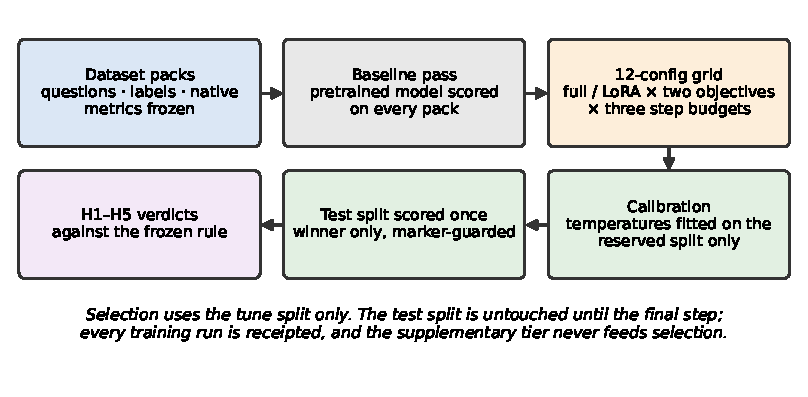
\includegraphics[width=\textwidth]{figures/fig_pipeline.pdf}
\caption{The frozen experiment pipeline. Dataset packs fix the questions, label spaces, and native metrics before any scoring; selection uses the tune split only; calibration is fitted on the reserved split after selection; and the official test split is scored exactly once, by the frozen winner.}
\label{fig:pipeline}
\end{figure}

\begin{table}[t]
\centering
\small
\caption{Measured metered GPU cost and operational characteristics.}
\label{tab:cost}
\begin{tabular}{ll}
\toprule
Item & Value \\
\midrule
Total metered GPU cost & \(\approx \$5.64\) \\
Rehearsal cost & \(\$0.17\) \\
Number of training runs & 29 \\
Pod rate & \(\$0.90\)/hour \\
Observed burn & \(\$0.897\)/hour \\
Inference latency & 0.16 s/item \\
Inference cost & \(\approx \$0.04\) per 1,000 predictions \\
Artifact size & \(\approx 805\) MB \\
\bottomrule
\end{tabular}
\end{table}

\subsection{MMFakeBench Grid Selection and Headline Test Result}
Table~\ref{tab:grid} ranks all 12 pre-registered grid configurations by tune macro-F1. The frozen winner is \( \texttt{full\_soft\_ce\_735} \), with tune macro-F1 0.7389 and tune accuracy 0.7429. Within this library's two objectives and under this recipe, soft-ce beats rlcd in all six matched pairs. Two failure modes are recorded: the full-rlcd training loss falls to approximately 0.00, and \( \texttt{lora\_rlcd\_735} \) collapses onto the original class with tune macro-F1 0.1946. Figure~\ref{fig:grid} presents the same selection as a heatmap.

\begin{table}[t]
\centering
\small
\caption{MMFakeBench grid selection on the tune split.}
\label{tab:grid}
\begin{tabular}{lcc}
\toprule
Configuration & Tune macro-F1 & Tune accuracy \\
\midrule
full\_soft\_ce\_735 & 0.7389 & 0.7429 \\
lora\_soft\_ce\_735 & 0.7187 & 0.7048 \\
full\_soft\_ce\_490 & 0.6598 & 0.6667 \\
lora\_soft\_ce\_245 & 0.6282 & 0.6571 \\
full\_rlcd\_735 & 0.6061 & 0.6190 \\
full\_soft\_ce\_245 & 0.5954 & 0.6000 \\
full\_rlcd\_490 & 0.5880 & 0.6000 \\
lora\_soft\_ce\_490 & 0.5726 & 0.5810 \\
full\_rlcd\_245 & 0.5667 & 0.5619 \\
lora\_rlcd\_245 & 0.4597 & 0.5905 \\
lora\_rlcd\_490 & 0.4505 & 0.6095 \\
lora\_rlcd\_735 & 0.1946 & 0.3333 \\
\bottomrule
\end{tabular}
\end{table}

\begin{figure}[t]
\centering
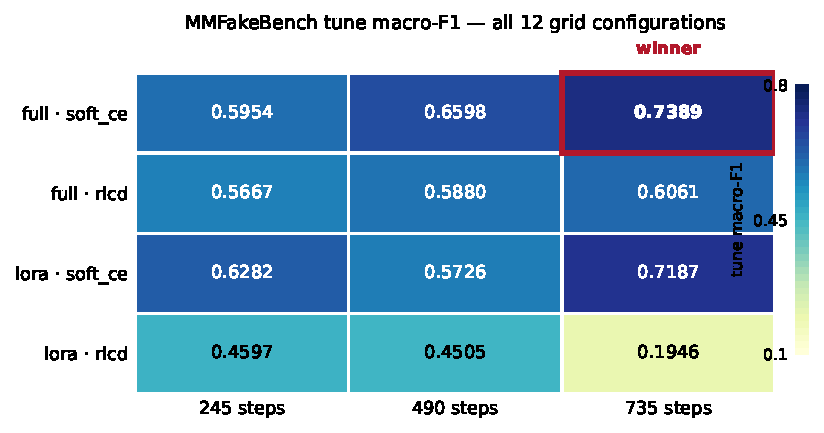
\includegraphics[width=\textwidth]{figures/fig_grid.pdf}
\caption{The MMFakeBench grid of Table~\ref{tab:grid} as a heatmap (tune macro-F1, \(n = 105\) tune items). The frozen winner, full encoder-plus-head with soft-ce at 735 steps (0.7389), is outlined.}
\label{fig:grid}
\end{figure}

The winner's per-class tune recalls are 0.656 for original, 0.969 for textual veracity distortion, 0.700 for visual veracity distortion, and 0.613 for mismatch. On the full validation split, the winner reaches accuracy 0.769 and macro-F1 0.7571, while the pretrained baseline under the same frozen wording reaches accuracy 0.293 and macro-F1 0.2079. Table~\ref{tab:mmfake} summarizes the headline test result. The official MMFakeBench test split is scored exactly once, on 9,999 paired rows with the single undecodable item excluded symmetrically from both arms. The winner reaches macro-F1 0.6020 versus baseline 0.2037. Paired resampling gives \(\Delta=+0.3983\), 95\% CI \([+0.3853, +0.4108]\). Every per-class recall improves.

The validation-to-test gap for the winner is large: 0.7571 validation macro-F1 versus 0.6020 test macro-F1. This is not a general test-time protocol failure, because the pretrained baseline is nearly flat across the same two splits (0.2079 validation versus 0.2037 test). Instead, the gap is consistent with selection on a small 105-item tune split and specialization to validation-style examples, while the official test contains 10,000 image--text pairs and a broader source/label composition. The per-class test recalls show that the largest remaining errors are on visual veracity distortion (0.512) and mismatch (0.422). By design, we do not use the test split to adapt the model or to select a different configuration after this single scoring. Figure~\ref{fig:headline} collects the before-and-after headline result for each of the three datasets on a common scale.

\begin{table}[t]
\centering
\small
\caption{Official MMFakeBench test result and per-class recalls.}
\label{tab:mmfake}
\begin{tabular}{lcc}
\toprule
Metric & Baseline & Winner \\
\midrule
Validation macro-F1 & 0.2079 & 0.7571 \\
Validation accuracy & 0.293 & 0.769 \\
Test macro-F1 & 0.2037 & 0.6020 \\
\midrule
Test recall: original & 0.213 & 0.617 \\
Test recall: textual & 0.524 & 0.834 \\
Test recall: visual & 0.026 & 0.512 \\
Test recall: mismatch & 0.135 & 0.422 \\
\bottomrule
\end{tabular}
\end{table}

\begin{figure}[t]
\centering
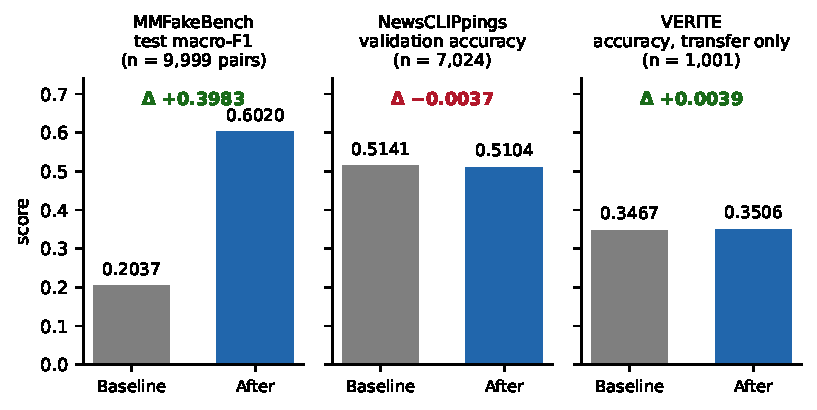
\includegraphics[width=\textwidth]{figures/fig_headline.pdf}
\caption{Before-and-after headline results, one panel per dataset, each on its native metric. Left: MMFakeBench test macro-F1, baseline 0.2037 to winner 0.6020. Centre: NewsCLIPpings validation accuracy, baseline 0.5141 to trained 0.5104, a null result. Right: VERITE accuracy under transfer only, baseline 0.3467 to 0.3506, near-flat. The three metrics are never averaged across datasets.}
\label{fig:headline}
\end{figure}

\subsection{NewsCLIPpings Trained Arm and Streamed Evaluation}
Table~\ref{tab:ncp} reports the NewsCLIPpings arm. The training carve uses only official train-split rows, so no validation or test rows enter training. The pretrained baseline scores 7,024 out of 7,024 streamed validation rows with accuracy 0.5141 and predicts falsified for 93\% of rows. The trained winner scores the same rows with accuracy 0.5104: a null result against this run's own baseline. Its pristine recall is 0.164, falsified recall is 0.857, binary-screen AUC is 0.529, and mean confidence is approximately 0.500. The trained model still predicts falsified for 84.6\% of pairs.

Although the trained arm makes fewer falsified calls than the baseline, it barely moves accuracy. With mean confidence near \(0.500\) and binary-screen AUC 0.529, the model does not learn a useful confidence-separated boundary and instead remains dominated by the falsified class. The pristine recall improves only from 0.084 to 0.164.

\begin{table}[t]
\centering
\small
\caption{NewsCLIPpings streamed validation results.}
\label{tab:ncp}
\begin{tabular}{lcc}
\toprule
Metric & Baseline & Trained winner \\
\midrule
Accuracy & 0.5141 & 0.5104 \\
Pristine recall & 0.084 & 0.164 \\
Falsified recall & 0.944 & 0.857 \\
Binary-screen AUC & 0.549 & 0.529 \\
\bottomrule
\end{tabular}
\end{table}

H2 is \textbf{NOT MET} under the re-aimed criterion. The trained winner's accuracy is only \(+0.2\) percentage points over October's 0.5083 and \(-0.4\) percentage points against this run's own baseline; at \(n=250\), the tune interval is roughly \([0.446, 0.570]\), so this margin is not a proven edge.\footnote{This run's baselines were measured with the frozen pack question wording; October's used different wording, and the baseline moved on identical rows (MMFakeBench validation accuracy \(0.320\rightarrow0.293\); NewsCLIPpings \(0.5083\rightarrow0.5141\); VERITE \(0.3566\rightarrow0.3467\)). October measured \(\pm0.03\) phrasing swings. Comparisons use one wording consistently or carry this footnote.} The temperature gate is mechanical: fitted NewsCLIPpings temperatures \([3.857, 2.100, 3.053]\) give held-out ECE 0.0127 versus raw ECE 0.0120, so the published NewsCLIPpings pack ships \(T=1.0\).

\subsection{VERITE Transfer}
Table~\ref{tab:verite} reports transfer-only results on 1,001 local rows of the official 1,000-item dataset. Our local extraction contains one additional row, so we score all local rows without ad-hoc filtering. No VERITE training is performed. The MMFakeBench winner transfers to VERITE with accuracy 0.3506, essentially flat relative to the baseline 0.3467. Per-class recalls are 0.808 for truthful, 0.148 for miscaptioned, and 0.086 for out-of-context. H3 is \textbf{NOT MET}; fine-tuning specialized the model for MMFakeBench's style of falsity and bought essentially nothing on VERITE's.

The transferred model differs from the baseline on 543 of 1,001 labels yet nets only \(+0.4\) percentage points accuracy and slightly lower macro-F1 (0.2798 versus 0.2819). This indicates label churn rather than useful transfer: the model is confident on truthful items but fails to separate VERITE's miscaptioned and out-of-context classes.

\begin{table}[t]
\centering
\small
\caption{VERITE transfer-only results.}
\label{tab:verite}
\begin{tabular}{lcc}
\toprule
Metric & Baseline & MMFakeBench winner transferred \\
\midrule
Accuracy & 0.3467 & 0.3506 \\
Macro-F1 & 0.2819 & 0.2798 \\
Truthful recall & 0.429 & 0.808 \\
Miscaptioned recall & 0.009 & 0.148 \\
Out-of-context recall & 0.612 & 0.086 \\
\bottomrule
\end{tabular}
\end{table}

\subsection{Calibration Analysis and H5}
Table~\ref{tab:calib} reports the three registered calibration measurements. On the reserved calibration split, fitted scaling reduces ECE from 0.2664 to 0.0865 and NLL from 2.64 to 0.61, with accuracy unchanged at 0.7048; H5 is \textbf{MET as registered}. However, when the fitted temperature \(T=8.4214\) is applied to the held-out MMFakeBench validation split, raw ECE 0.1056 worsens to 0.3955. A split-half fit on the same validation data yields \(T\approx1.65\), and held-out ECE improves from 0.0994 to 0.021. A full-validation fit gives \(T\approx1.6\).

\begin{table}[t]
\centering
\small
\caption{Calibration measurements under distribution shift.}
\label{tab:calib}
\begin{tabular}{lcc}
\toprule
Setting & Raw ECE & Fitted ECE \\
\midrule
Registered calibration split & 0.2664 & 0.0865 \\
Held-out validation, using split-fitted \(T=8.4214\) & 0.1056 & 0.3955 \\
Split-half validation, using half-fitted \(T\approx1.65\) & 0.0994 & 0.021 \\
\bottomrule
\end{tabular}
\end{table}

The disposition is as executed: H5 stands as registered with this qualification, the published MMFakeBench pack ships \(T=1.0\), and \(T\approx1.6\) is documented only as a deployment-calibration alternative. This is a concrete instance that a temperature is a property of model-times-distribution, not a model constant \citep{Guo2017CalibrationModern, Ovadia2019CanYou, Minderer2021RevisitingCalibration}.

\subsection{Supplementary Ablations, Protocol Audit, and Competitive Position}
The supplementary ablation tier runs after selection and never feeds selection, calibration, or test-once scoring. A second seed of the winner recipe reaches 0.7320, so the winner is not a lucky-seed artifact at the tune level. Encoder learning-rate variants score 0.7178, 0.6871, 0.6438, and 0.6217. LoRA rank r8 reaches 0.7037 at 490 steps, while r32 collapses or diverges: 0.1168 at 490 steps and 0.2244 at 735 steps with training loss rising from 0.762 to 1.070. At this data scale, higher LoRA rank is a stability hazard under the standard recipe. Head-only fine-tuning scores at most 0.4899 and is never described as a linear probe. The data-size curve collapses at 122 training items \((0.1168)\), improves to 0.3670 at 245 items, and reaches 0.6598 at 490 items, indicating a minimum-data cliff. Figure~\ref{fig:ablations} plots the data-size curve and the LoRA rank ladder.

\begin{figure}[t]
\centering
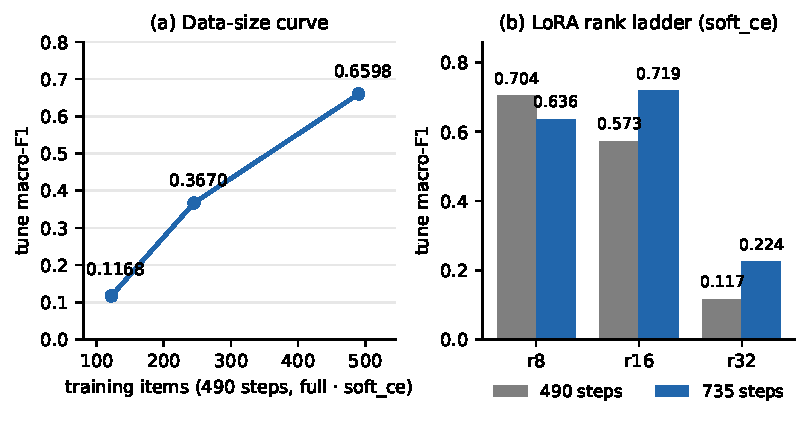
\includegraphics[width=\textwidth]{figures/fig_ablations.pdf}
\caption{Supplementary-tier behaviour on the MMFakeBench tune split. (a) The data-size curve at 490 steps: performance collapses at 122 training items (0.1168), recovers at 245 items (0.3670), and reaches 0.6598 at 490 items. (b) The LoRA rank ladder under soft-ce: rank 8 and rank 16 remain trainable at both step budgets, while rank 32 collapses. The rank-16 column is the main grid's LoRA arm.}
\label{fig:ablations}
\end{figure}

We did not retrain standard vision-language baselines such as CLIP, VisualBERT, or LXMERT under the frozen 490-example protocol. This is a pre-registered single-model audit: adding multiple model families would produce a benchmark sweep rather than the receipted protocol study we froze. A benchmark sweep would also need to choose one of several incompatible protocols; since protocol fragmentation is one of the paper's findings, mixing new retrained baselines into only one of those protocols would not resolve the fragmentation and could be misleading. For external systems we therefore use published Protocol A results and label every protocol rather than creating new mixed comparisons.

Table~\ref{tab:protocol} separates Protocol A official-test results from non-comparable regimes. On Protocol A, LAYA-Vision trails only the frontier-model agent system and leads every fine-tuned system reported. Other published numbers use validation, binary, retrieval, or private re-split protocols and are not directly comparable.

\begin{table}[t]
\centering
\small
\caption{Protocol-labelled MMFakeBench comparison.}
\label{tab:protocol}
\begin{tabular}{lcc}
\toprule
System & Protocol & Macro-F1 \\
\midrule
GPT-4V Standard & A: official test & 48.8 \\
GPT-4V + MMD-Agent & A: official test & 61.5 \\
LLaVA-1.6-34B Standard & A: official test & 25.7 \\
SCPO & A: official test, Top-1 extraction & 57.3 \\
DeceptionDecoded & A: split unverified & 58.66 \\
LAYA-Vision (this study) & A: official test & 60.20 \\
\midrule
\multicolumn{3}{l}{\textit{Not Protocol A: not directly comparable}} \\
MERIT/MIRAGE & binary, validation, retrieval & 81.65 \\
T2Agent & validation, test-time search & 75.9 \\
MM-VeriAgent & private re-split & 71.5 \\
AgentM3D & validation & 62.6 \\
LRQ-FACT & validation & 71.6 \\
\bottomrule
\end{tabular}
\end{table}

Cost estimates for frontier systems are marked as estimates, not measurements. Scoring the 10,000-item test once via a GPT-4V-class API is estimated at about \$155, and an agent framework at roughly \$450--750. These are about 1,000 times the per-item cost of the LAYA forward pass.

\section{Conclusion}
\label{sec:conclusion}
%%%%%%%%% CONCLUSION %%%%%%%%%%
We presented a pre-registered fine-tuning study of LAYA-Vision, a 201M-parameter typed-decision model, under a frozen protocol across MMFakeBench, NewsCLIPpings, and VERITE. The contribution is not a new architecture or training algorithm; it is a pre-registered, receipted, low-cost evaluation procedure that makes dataset conditionalities and benchmark shortcuts visible. On the official MMFakeBench test, fine-tuning on 490 examples reaches 0.6020 macro-F1 with low measured metered GPU cost and zero external dependencies. The same recipe is dataset-conditional: it yields a large MMFakeBench gain, a null NewsCLIPpings result, and flat VERITE transfer. Methodologically, the study contributes a 0.9150 metadata leakage ceiling, evidence that calibration temperatures are distribution-specific, a protocol audit that separates official-test results from retrieval, validation, and private re-split regimes, and a complete metered GPU cost and deviations ledger. The result is a fully reproducible, low-cost pre-registered study with public checkpoints and a demo, reported without softening negative outcomes.

%%%%%%%%% REFERENCES %%%%%%%%%%
\bibliography{references}
\bibliographystyle{iclr2025_conference}
%%%%%%%%% REFERENCES %%%%%%%%%%

%%%%%%%%% Appendix %%%%%%%%%%
\appendix
\section{Pre-registration, Hypotheses, Amendments, and Deviations}
\label{app:protocol}
The five pre-registered hypotheses and their binary verdicts are as follows.
\begin{itemize}
    \item \textbf{H1 (MMFakeBench gain):} MET on test. The winner improves test macro-F1 from 0.2037 to 0.6020; paired-resampling 95\% CI lower bound is \(+0.3853\), and no per-class recall drops.
    \item \textbf{H2 (NewsCLIPpings trained arm):} NOT MET. Trained accuracy 0.5104 is outside the \(0.55\)--\(0.65\) band and not at least \(+6.24\) percentage points over the October baseline 0.5083.
    \item \textbf{H3 (VERITE transfer):} NOT MET. Transfer accuracy 0.3506 is outside the \(0.38\)--\(0.48\) band.
    \item \textbf{H4 (recall floor):} MET. Minimum per-class tune recall of the winner is 0.613.
    \item \textbf{H5 (calibration):} MET as registered, with the qualification in Section 4.5.
\end{itemize}

Design amendments are disclosed as follows. Amendment (b) keeps the vision tower frozen in both arms because the library's training loop cannot unfreeze it; the full arm therefore trains the language encoder plus decision head only. Amendment (c) adds a NewsCLIPpings training arm carved from its official train split, with its H2 criterion re-aimed at that arm. Amendment (d) adds the supplementary ablation tier after the registered core; its receipts are isolated and never feed selection, calibration, or test-once scoring.

The following deviations are recorded faithfully. (1) Frozen vision tower per amendment (b). (2) NewsCLIPpings evaluation by streaming, with no archived image storage for evaluation. (3) NewsCLIPpings trained arm and saved training-subset exception. (4) Notebook-only execution on the run machine's Jupyter kernel. (5) Supplementary ablation tier. (6) NewsCLIPpings selection metric uses the native question form only because the two question forms have flipped label indices. (7) Inert tag in the executed NewsCLIPpings training cell, which never passed the dataset parameter; results are unaffected. (8) Carve manifest erratum: the manifest label reads 2,000 train items while the files contain 2,001. (9) VERITE transfer defect with two layers: the pack registry initially pointed to the base checkpoint, and a checkpoint-blind output-directory reuse cache defeated the first fix; a clean re-run protocol corrected this. (10) Calibration qualification in Section 4.5. (11) PASS 2 stream engine change after 709 serial rows; the parallel engine was restarted from row 0 and an equivalence gate on 120 shared items found zero label mismatches and bitwise identical probabilities.

The full receipt bundle includes timestamped pre-registration, amendments, deviations, and per-configuration receipts. To preserve double-blind review, no public checkpoint, demo, or receipt URLs are disclosed in this submission; the artifact pointers are recorded in the receipt bundle and omitted here. The metadata leakage audit uses only \( \texttt{text\_source} \) and \( \texttt{image\_source} \), and scores 0.9150 macro-F1 on tune, and 0.9150 accuracy / 0.8510 macro-F1 on test.

\section{Supplementary Tables and Reproducibility Checklist}
\label{app:tables}
For reproducibility, Table~\ref{tab:ablation} summarizes the supplementary ablation tier. The binding labelling rules are: LoRA learning rate is \( \texttt{lr\_lora}=0.001\); head-only fine-tuning is never called a linear probe; VERITE is described as 1,001 local rows of the official 1,000-item dataset; baseline comparisons carry a wording footnote; rlcd claims are scoped to this library's two objectives and this recipe; the full arm is described as encoder-plus-head with the vision tower frozen. Artifact pointers for public checkpoints and the demo are omitted from this draft.

\begin{table}[t]
\centering
\small
\caption{Supplementary ablation tier on MMFakeBench tune split.}
\label{tab:ablation}
\begin{tabular}{lc}
\toprule
Configuration & Tune macro-F1 \\
\midrule
Second seed, winner recipe & 0.7320 \\
Encoder LR \(2\times10^{-5}\), 735 steps & 0.7178 \\
Encoder LR \(2\times10^{-5}\), 490 steps & 0.6871 \\
Encoder LR \(5\times10^{-6}\), 735 steps & 0.6438 \\
Encoder LR \(5\times10^{-6}\), 490 steps & 0.6217 \\
LoRA r8, 490 steps & 0.7037 \\
LoRA r8, 735 steps & 0.6362 \\
LoRA r32, 735 steps & 0.2244 \\
LoRA r32, 490 steps & 0.1168 \\
Head-only soft-ce, 490 steps & 0.4238 \\
Head-only soft-ce, 735 steps & 0.3098 \\
Head-only rlcd, 735 steps & 0.4899 \\
Head-only rlcd, 490 steps & 0.2590 \\
Data size 122, 490 steps & 0.1168 \\
Data size 245, 490 steps & 0.3670 \\
Data size 490, 490 steps & 0.6598 \\
\bottomrule
\end{tabular}
\end{table}

\section{Execution Evidence}
\label{app:evidence}
The study was executed as a single notebook run, and the notebook is the run record: anyone can check each stage's input, process, and output in the executed cells without further explanation. Figure~\ref{fig:collage} reproduces verbatim excerpts of that record, covering the frozen configuration, the environment and GPU check, the grid results, winner selection, the test-once guard, and the final hypothesis verdicts.

\begin{figure}[p]
\centering
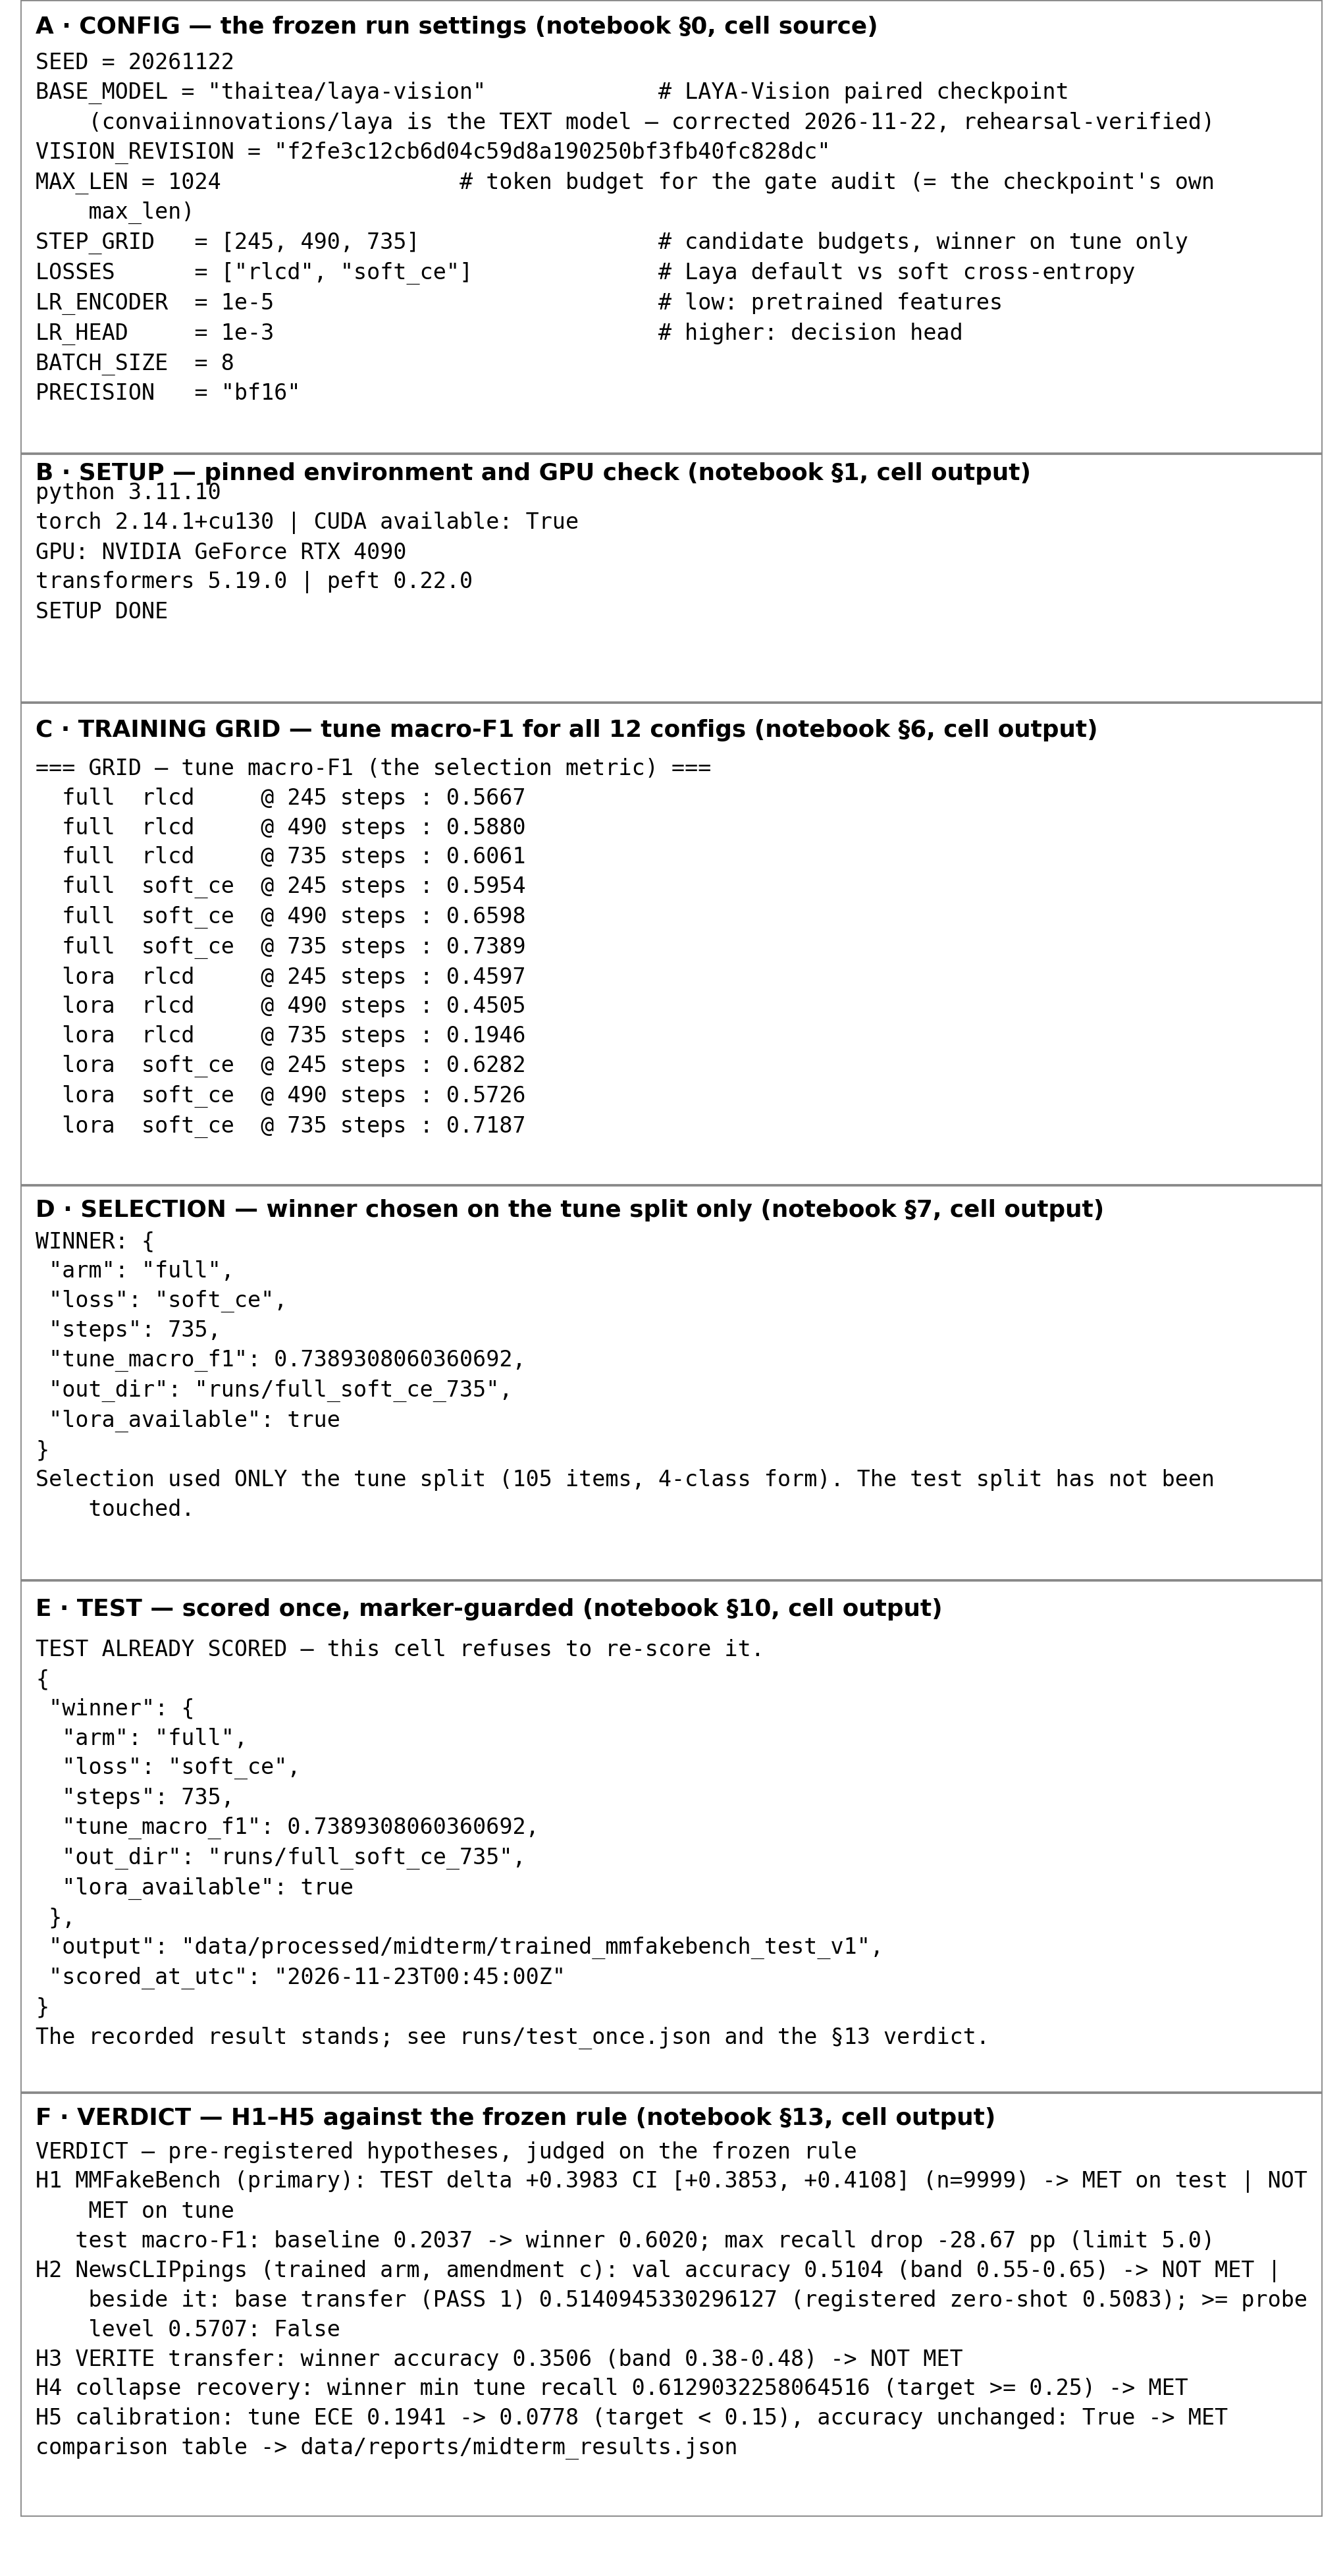
\includegraphics[width=\textwidth,height=0.89\textheight,keepaspectratio]{figures/collage_colab.png}
\caption{Execution evidence from the run notebook, reproduced verbatim. Panels show, in order: the frozen configuration; the pinned environment and GPU check; the training grid's tune macro-F1 table; winner selection on the tune split; the test-once marker, which refuses any re-scoring; and the H1--H5 verdicts computed against the frozen rule. Repeated library deprecation warnings are omitted from the excerpts; no values are altered.}
\label{fig:collage}
\end{figure}

\section{Code Appendix: Pseudocode}
\label{app:code}
This appendix compresses the study's own code into pseudocode. Each block is a faithful compression of the real code named in its subsection: the same steps in the same order, with the source's named constants, and no invented steps. The source files are versioned with this paper in the code folder of the study repository. Sections~\ref{app:code-verifier} and~\ref{app:code-parallel} describe components of the reported study. Section~\ref{app:code-v2} documents two components built after the study closed, for the follow-on probe; they are labelled as such, and no result reported above depends on them.

\subsection{The VisualNews Stream Verifier}
\label{app:code-verifier}
The verifier (\texttt{visualnews\_stream.py}) is the only route by which NewsCLIPpings evaluation images reach the model. The VisualNews archive is streamed once over HTTP and images are never written to disk. Member names in the archive are unreliable at source-dependent rates (payloads behind \texttt{.jpg} names are sometimes GIF, PNG, or BMP), so every decision is made on the decoded bytes, never on the extension. Only integrity failures skip; dataset properties (non-JPEG payloads, palette or RGBA modes, progressive JPEGs, animated images) never do.

{\footnotesize\begin{verbatim}
function verify_image_bytes(data):        # -> (ok, reason, image)
    if data is empty:
        return (False, "empty_member", None)
    try:
        img <- PIL open(data)      # format read from the bytes,
                                   # never from the member name
        if img.width * img.height > HARD_PIXEL_LIMIT:
            return (False, "oversize_dimensions", None)
                                   # 200,000,000 declared pixels:
                                   # refuse BEFORE allocating the
                                   # decode buffer
        img.load()                 # full decode, not a header
                                   # sniff: truncated payloads that
                                   # pass open() fail here. Animated
                                   # images decode frame 0, which is
                                   # what the pipeline judges.
    except any error e:
        return (False, reason_of(e), None)
                                   # "truncated" if the error
                                   # reports truncation, else
                                   # "decode_error"
    if img.width < MIN_DIMENSION or img.height < MIN_DIMENSION:
        return (False, "degenerate_dimensions", None)   # 8 pixels
    if img.mode is palette and it carries byte transparency:
        img <- img.convert("RGBA") # per PIL's own guidance, so
                                   # transparency is handled
    return (True, None, img.convert("RGB"))
\end{verbatim}}

{\footnotesize\begin{verbatim}
procedure stream_verified(source, referenced, on_image):
    wanted <- { normalize(p) : p  for p in referenced }
    ledger <- new SkipLedger
    ledger.note_referenced(each referenced path)
    stream <- open_stream(source)
      # a URL is fetched through a parallel range reader (range
      # segments served strictly in order; if the server does not
      # honour Range, fall back to a plain single stream); a local
      # path or an open file object is used directly. Socket reads
      # carry a 120 s inactivity timeout: a stalled stream raises.
    seen <- {}
    for member in tar_stream(stream, mode = "r|*"):
                                   # one pass, members consumed in
                                   # archive order
        if member is not a regular file: continue
        original <- wanted.get(normalize(member.name))
        if original is absent: continue
                                   # unreferenced: its payload is
                                   # never read; the stream reader
                                   # discards it as it advances
        seen.add(normalize(member.name))
        ledger.note_seen(original)
        data <- read member payload (empty bytes if none)
        (ok, reason, image) <- verify_image_bytes(data)
        if not ok:
            ledger.skip(original, reason); continue
        ledger.note_verified(original)
        results.append({ path: original,
                         prediction: on_image(original, image) })
    for each referenced path never seen in the stream:
        ledger.note_missing(path)
    return (results, ledger.summary())
    # summary(): referenced / seen / verified / skipped counts,
    # skip-reason counts, missing count, and the same accounting
    # per source (bbc, guardian, usa_today, washington_post,
    # other). A bad member never raises; only stream-level
    # failure raises, so the caller can restart the pass.

normalize(p): backslashes -> "/"; strip leading "./" segments
    and a leading "origin/" prefix. Applied identically to tar
    member names and to referenced paths before matching.
\end{verbatim}}

\subsection{The Parallel Stream Engine and Its Equivalence Gate}
\label{app:code-parallel}
The streamed validation pass of the NewsCLIPpings trained arm (PASS~2) was restarted on a parallel engine, because the serial pass is bounded by a single sequential tar traversal. The measurement procedure is identical to the serial engine's: same verifier semantics, same checkpoint, same pack questions, same temperatures, same prediction call, same row schema. Only execution concurrency changed, and the parallel engine was trusted only after the equivalence gate below passed. The worker processes live in \texttt{parallel\_stream\_engine.py}; the orchestration and the gate live in \texttt{parallel\_gate\_cell.py}, exported from the executed notebook cell.

{\footnotesize\begin{verbatim}
procedure run_parallel_pass(pack, checkpoint, rows, out_dir):
    groups <- rows grouped by image member (one image, many rows)
    saved  <- prediction rows already in out_dir (resume support)
    done   <- ids of saved rows with status ok
    start processes under the SPAWN context (never fork: CUDA
    cannot be re-initialised in a forked subprocess):
        1 reader process, 6 decode processes, 4 inference
        processes; queues byte_q (reader -> decoders), img_q
        (decoders -> inferers), evt_q (all -> coordinator)

    reader: stream the tar once, in archive order; for each
        member whose normalised name is wanted and not yet sent,
        emit a "seen" event and put (path, payload bytes) on
        byte_q; at end of stream signal reader_done (on stream
        failure, signal aborted instead)
    decoder (x6): loop on byte_q (stop on sentinel):
        verify_image_bytes(bytes); on failure emit skip(path,
        reason); on success emit verified(path) and put (path,
        image relayed as lossless PNG bytes) on img_q;
        then signal decode_done
    inferer (x4): load the checkpoint once; loop on img_q (stop
        on sentinel): for each row of this image whose id is not
        in done, predict with the pack's questions and
        temperatures and emit the item record on evt_q (status
        ok; blocked if the row's text is missing; error, with
        the exception counted, if predict raises);
        then signal infer_done
    coordinator (the single writer): consume evt_q; update the
        SkipLedger from seen / verified / skip events; append
        each item record to paired.predictions.jsonl, never
        writing an id already saved; when reader_done arrives,
        stop the decoders; when all decoders are done, stop the
        inferers; finish when all inferers report done
    dead-worker guard: if every inference process has exited
        without reporting done, abort loudly (the pipeline can
        never finish); likewise if all processes exit before
        their completion signals
    on abort: raise; scored rows stay on disk and resume
    reconciliation (only when not aborted): members skipped by
        the verifier or missing from the stream get explicit
        blocked rows for their unscored rows (reason recorded),
        so every referenced row is accounted for exactly once;
        metrics and per-source accounting follow from the
        completed prediction file

equivalence gate (runs before the full parallel pass):
    shared <- items scored by BOTH the preserved serial partial
              and a parallel run limited to the serial-scored
              members (serial file order is tar order, so the
              gate reads the tar head only)
    require |shared| >= 100
    require predicted labels identical on every shared item
    require max |p_parallel - p_serial| <= 0.001 on shared items
    any failure -> abort the restart; resume the serial pass
    executed run: 120 shared items, zero label mismatches, zero
    measured probability drift; the gate passed
\end{verbatim}}

\subsection{Post-Study Additions (v2): EvidenceGate and the Retrieval Repair}
\label{app:code-v2}
The two components below were built after this study closed, for the follow-on retrieval probe. They are part of the codebase but not of the study reported above: no result in this paper uses them. They are recorded here so the code record is complete.

EvidenceGate is a pluggable per-item state machine around the paired judgement: it routes an item to a pair-only judgement or to a retrieve-then-judge path. Its configuration lives in the pack (\texttt{mode} in \{off, on, auto\}); with the gate off, behaviour is the pipeline of this study exactly. The specification is versioned in the probe design document.

{\footnotesize\begin{verbatim}
states:
    INTAKE    item + pack + checkpoint enter; the image is
              verified under the discipline of the verifier
              above
    ROUTE     the routing decision is computed and recorded,
              with its reason
    PAIR_ONLY the paired judgement of this study: pack questions
              verbatim, caption-only context. In mode auto its
              verdict is provisional.
    RETRIEVE  the retrieval pipeline below produces the item's
              frozen evidence bundle
    JUDGE     the model judges image + caption + evidence
              context with the registered evidence questions
    ARBITRATE the arbitration rule of this study: the choice
              verdict headlines; choice/noul disagreement gives
              verdict "uncertain"
    DONE      terminal: exactly one output record for the item
    ABSTAIN   terminal, unscored: integrity skip or
              unrecoverable model failure; counted in the run
              accounting. Distinct from "uncertain", which is a
              scored outcome produced by arbitration.

transitions and guards:
    INTAKE -> ROUTE        image verified; pack + gate load
    INTAKE -> ABSTAIN      verification fails (skip ledgered),
                           or pack/checkpoint cannot be loaded
    ROUTE -> PAIR_ONLY     mode off, or mode auto (pair first)
    ROUTE -> RETRIEVE      mode on
    PAIR_ONLY -> ARBITRATE mode off; or mode auto and the
                           trigger does not fire. Headline is
                           the pair-only verdict.
    PAIR_ONLY -> RETRIEVE  mode auto and the trigger fires; the
                           provisional pair-only verdict is kept
                           in the record as the control
    RETRIEVE -> JUDGE      bundle holds at least one passage
    RETRIEVE -> ARBITRATE  bundle empty or unusable; the
                           pair-only control verdict headlines
                           and the trace is flagged
    JUDGE -> ARBITRATE     always; headline is the evidence
                           verdict
    ARBITRATE -> DONE      always
    any -> ABSTAIN         predict raises, or a bundle's
                           snapshot hash check fails (never
                           judge on unverified evidence)

trigger (mode auto): the pair-only pass returns the choice
    distribution P and the noul fake probability q.
    margin       = largest P - second-largest P
    disagreement = (choice headline is fake-side) != (q >= 0.5)
    RETRIEVE fires iff margin < 0.20 or disagreement
    (both thresholds are registered knobs, frozen before any
    results; the trigger measurements are recorded in every
    item's state trace whether or not retrieval fires)

RETRIEVE, five steps (the search index is transport only: it
    fetches; it does not rank, select, or decide):
    1. extraction (deterministic): named entities plus noun
       chunks from the caption; variant A queries are built
       from these spans by a fixed template
    2. harness query expansion: a small model returns a
       one-line claim restating the caption and 2-3 further
       queries (variant B); it never sees gold labels or the
       image, and the claim text is used for queries only,
       never placed inside the judge's evidence block
    3. transport: both variants' queries issued to the search
       index (20 s per-query timeout); results unioned and
       deduplicated by URL; every result, used or not, is
       written into the snapshot with its URL, title, snippet,
       engine, timestamp, query, and variant
    4. triage: fact-check domains on the versioned
       contamination list and the item's own source article
       are excluded from the headline pools (kept in the
       snapshot, counted); results that merely repeat the
       caption's own claim are down-ranked, not deleted, and
       near-duplicate clusters collapse to their best member;
       survivors are ordered by whether they bear on the
       claim's checkable content (people, places, events,
       dates)
    5. selection + freeze: the top 5 passages, at most 600
       characters each, are selected in triage order and
       packed under the token budget; the bundle is written
       to disk and hashed (SHA-256); from this moment the
       item's evidence is fixed
\end{verbatim}}

The retrieval repair loop repaired a silent instrument failure in the probe's batch retrieval: concurrent query load tripped the search engine's suspension, and empty result lists were recorded as if they were results for most item-variants. The repair re-runs only the failed pairs, serially, with the items' frozen query lists and the same contamination rules.

{\footnotesize\begin{verbatim}
procedure repair_retrieval(items, raw_in, harness_in,
                           raw_out, harness_out):
    repair_list <- every (item, variant) whose recorded pool
                   size is 0
    new_raw <- all raw records except stale repair records for
               pairs in repair_list (untouched pairs are copied
               through verbatim; the original files remain as
               the pre-repair record)
    streak <- 0
    for each (item, variant) in repair_list:
        pool <- {}
        for q in the item's frozen query list (unchanged):
            results <- search(q)     # one query at a time; up
                                     # to 3 attempts, waiting
                                     # between attempts
            if results is empty:
                streak <- streak + 1
                if streak reaches 10:      # circuit breaker
                    sleep 240 s            # engine suspension:
                    streak <- 0            # pause, then resume
            else:
                streak <- 0
            for each result, in rank order:
                build its record (query, rank, URL, title,
                snippet, engine, score, published date,
                fact-check-domain flag, self-hit flag,
                timestamp, repair flag set)
                append the record to new_raw
                keep the best-scoring record per URL in pool
            sleep 1 s                # the disciplined rate
        record the item's new pool size for this variant
        try: re-run triage and passage selection on the pool;
             store the triage record and both passage sets
             (headline: fact-check excluded; second: included)
        on failure: store the error and empty passage sets,
             and count the failure
        mark the item repaired, with the repair timestamp
        flush both output files   # per-pair checkpoint: outputs
                                  # are rewritten atomically
                                  # after every pair, so a
                                  # stopped run loses nothing
    flush; write the run statistics (pairs repaired, harness
    calls and failures, balance before and after, spend)
    # pairs still empty after the repair are reported as
    # retrieval-failed, a different state from a genuine
    # no-evidence item, whose search ran and found nothing
\end{verbatim}}

%%%%%%%%% Appendix %%%%%%%%%%

\end{document}